\documentclass{beamer}
\usepackage{tikz}
\usepackage{graphicx}
\usetheme{metropolis}
\usepackage{lmodern}
\usepackage{amsmath}
\usepackage{mathrsfs}
\usepackage{pdfpages}
\usepackage[backend=biber, style=science]{biblatex}
\addbibresource{/Users/fergusbarratt/bibTex/library.bib}
\graphicspath{ {../../../Images/Presentation/} }

\title{The Dissipative-Driven Jaynes-Cummings System}
\date{\today}
\author{Fergus Barratt}

\begin{document}
\setbeamercolor{block title}{bg=}
\setbeamercolor{block body}{bg=}
\setbeamercolor{background canvas}{bg=}
\maketitle

\begin{frame}

    \frametitle{Superconducting circuit QED}         

    \begin{itemize}

        \item CQED is a promising paradigm for the implementation of 
                quantum computers. 
        \item One critical component is the qubit implementation.
        \item CQED the canonical example is the Josephson junction 
                qubit, which come in three kinds, charge, flux, and 
                phase\footfullcite{Makhlin2001}. 
        \item Decoherence is a key problem.
        \item One suggestion is the \emph{transmon}
                \footfullcite{Blais2004a} 
                a compound system of Josephson qubits.

    \end{itemize}

\end{frame}

\begin{frame}
    \frametitle{Cooper Pair Box (CPB)}

    \begin{columns}[c]
        \begin{column}{0.4\linewidth}
            \includegraphics[scale=0.8]{cpb.png}
        \end{column}
        \begin{column}{0.6\linewidth}
            \begin{itemize}

                \item The CPB is a charge qubit implementation where 
                    information is encoded in the occupation of a 
                    superconducting `island'

                \item The CPB has Hamiltonian 
                    $
                    \mathscr{H} = 4 E_c \left(N - N_g\right)^2 
                    - E_J \cos \varphi
                    $
                    with N the difference in pair occupation, 
                    $\varphi$ the gauge-invariant phase difference
                
            \end{itemize}
        \end{column}
    \end{columns}

\end{frame}
\begin{frame}

    \frametitle{The Transmon}

    \begin{columns}[c]

    \begin{column}{0.4\linewidth}

            \begin{block}{}
                \vspace{-0.5cm}
    \includegraphics[scale=0.25]{transmon.png}
            \end{block}

    \end{column}

    \begin{column}{0.6\linewidth}
    
        \begin{itemize}
            
            \item The transmon consists again of a single island, 
                    coupled by two Josephson junctions with an
                    additional parallel capacitance. 
            \item Figure of merit for qubit candidates is level 
                    anharmonicity. 
            \item Increasing anharmonicity increases noise.
            \item The transmon can be operated in a regime where noise 
                    can be suppressed with small anharmonicity losses. 
                    
        \end{itemize}

    \end{column}

    \end{columns}

\end{frame}
\begin{frame}

    \frametitle{Two-Level approximation}

    \begin{columns}[c]

        \begin{column}{0.5\linewidth}

            \begin{block}{}
    \vspace{-.7cm}
    \includegraphics[scale=0.25, angle=-90, origin=c]{anharmonicity.pdf}
            \end{block}

        \end{column}
        \begin{column}{0.5\linewidth}

            \begin{itemize}
                \item If we increase the anharmonicity we can 
                        have negligible population of higher levels 
                        and an effective qubit.
                \item We put the transmon in a cavity and couple 
                        the preferred mode to light.
                \item This is the Jaynes-Cummings model of 
                        Quantum Optics. 
            \end{itemize}

        \end{column}
    \end{columns}

\end{frame}
\begin{frame}

    \frametitle{The Jaynes-Cummings Model}

    \begin{center}
        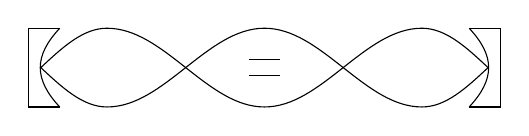
\begin{tikzpicture}[xscale=2]
                \draw (0, 1) -- (0, 0);
                \draw (0, 1) -- (0.2, 1);
                \draw (0, 0) -- (0.2, 0);
                \draw (0.2, 0) to [out=-245, in=245] (0.2, 1);

                \draw (3, 1) -- (3, 0);
                \draw (2.8, 1) -- (3, 1);
                \draw (2.8, 0) -- (3, 0);
                \draw (2.8, 0) to [out=-295, in=295] (2.8, 1);

                \draw (0.08, 0.5) sin (0.5, 1) cos (1, 0.5) sin (1.5, 0) cos (2, 0.5) sin (2.5, 1) cos (2.92, 0.5);

                \draw (0.08, 0.5) sin (0.5, 0) cos (1, 0.5) sin (1.5, 1) cos (2, 0.5) sin (2.5, 0) cos (2.92, 0.5);

                \draw (1.4, 0.4) -- (1.6, 0.4);
                \draw (1.4, 0.6) -- (1.6, 0.6);
        \end{tikzpicture}
    \end{center}

    Single cavity mode interacting with two level system in the RWA.
    Add coherent drive, dissipation via cavity loss $\kappa$ \& 
    spontaneous emission rate $\gamma$

    \begin{block}{Interaction Hamiltonian}
        $
        \mathscr{H} = \hbar \delta_{cd} a^\dagger a + 
        \hbar \delta_{qd}\sigma_+ \sigma_- + 
        \hbar g ( a \sigma_+ + a^\dagger \sigma_- ) + 
        \hbar \xi (a + a^\dagger) 
        $
    \end{block}

    \begin{block}{Master Equation}
        $
        \dot{\rho_S} = \frac{i}{\hbar} [ \mathscr{H}, \rho_S ] +
        \mathscr{L}_{\gamma} [\rho_S] + \mathscr{L}_{\kappa}[ \rho_S ]
        $
    \end{block}

\end{frame}
\begin{frame}

    \begin{block}{Resonant}
        $
        \delta_{cq} = \delta_{cd}=0
        $
        \footfullcite{Alsing1990}
        \footfullcite{Carmichael2015}
    \end{block}

\end{frame}
\begin{frame}

    \includepdf{resonant.pdf}

\end{frame}
\begin{frame}

    \begin{block}{Dispersive}
        $
        \gamma \ll \kappa \ll g \ll \delta_{cq} \ll \omega_c
        $
        \footfullcite{Bishop2010}
    \end{block}

\end{frame}
\begin{frame}

    \frametitle{Effect of the detuned qubit}

    \begin{block}{Exact Hamiltonian}

        $
        \mathscr{H} = \hbar \delta_{cd} a^\dagger a + 
        \hbar \delta_{qd}\sigma_+ \sigma_- + 
        \hbar g ( a \sigma_+ + a^\dagger \sigma_- ) 
        $

    \end{block}
    \begin{block}{Dispersive Hamiltonian}
        we expand in $\frac{g}{\delta_{cq}}$ and transform with 
        $
        U = \exp \left \{\frac{g}{\delta_{cq}} 
            ( a \sigma_+ - a ^ \dagger \sigma_- ) \right \}
        $

        $ 
        U\mathscr{H}U ^ \dagger \approx \hbar 
        \left\{ \omega_c + \frac{g^2}{\delta_{cq}} \sigma_z \right\}
        a ^ \dagger a + 
        \frac{\hbar}{2} \left\{ \omega_q + \frac{g^2}{\delta_{cq}} \right\}
        \sigma_z 
        $
    
    The qubit pulls the cavity frequency (and the cavity the qubit)

    \end{block}

\end{frame}
\begin{frame}

    \frametitle{Why the dispersive regime?}

    \begin{block}{Qubit Readout \& Control}
        \begin{itemize}

            \item We can read out the state of the qubit 
                    without destroying it\footfullcite{Blais2004a}. 
            \item In the dispersive regime the qubit pulls the 
                    cavity frequency up or down based on its state.
            \item Driving the cavity at what was cavity 
                    resonance encodes the qubit superposition 
                    in the transmitted photons. 
            \item Driving the qubit can be used to coherently 
                    control the qubit state. 

        \end{itemize}
    \end{block}

\end{frame}
\begin{frame}

    \frametitle{The Duffing Oscillator}

    \begin{columns}[c]

        \begin{column}{0.5\linewidth}
            \includegraphics[scale=0.5]{leaf.png}
        \end{column}

        \begin{column}{0.5\linewidth}
            \includegraphics[scale=0.4]{scurve.png}
        \end{column}

    \end{columns}

    \begin{block}{}
        \begin{itemize}

            \item Unlike the Duffing nonlinearity 
                \footfullcite{Drummond1979},
                the JC nonlinearity softens with increasing drive
                \footfullcite{Bishop2010}.

        \end{itemize}
    \end{block}

\end{frame}
\begin{frame}

        \includepdf{dispersive.pdf}

\end{frame}
\begin{frame}

    \printbibliography

\end{frame}

\end{document}
